% !TeX root = ../0_Manuscript.tex

\section{Enhanced BBI platform in a fault attack context \ddc}
\label{chap:2_goodPractices;sect:enhancedBBIGiraudAttack}
Now that we have seen with simple actual experiments the benefits of the proposed enhanced \bbi platform, let us linger on further experiments to verify more thoroughly the soundness of these enhancements.
To that end, I performed a differential fault attack on our IC target.
More specifically, a constraining fault attack requiring single bit faults on one or more bytes working on an AES cryptographic core, introduced by C. Giraud \cite{giraudDfa} in 2004.
In the first place, we are going to discuss in details the core of the attack.
Afterward, I will describe the IC target, its characteristics, and its operating conditions for the experiments.
Then, I will introduce experiments we developed to perform preliminary measurements to the attack, accelerating the search of points of interests on the IC.
Next, we will discuss the practical attack results.
Eventually, we will draw conclusions on the various observations.

    \subsection{Giraud's DFA detailed description \ddc}
    When Giraud's paper \cite{giraudDfa} was published in 2004, no existing DFA was capable of attacking an AES algorithm.
    In this context, they proposed two types of DFA on AES, in order to cover various fault types one can induce on secured ICs.
    In this thesis, I focused on the first fault model, consisting in inducing single bit faults, therefore, this is the one we are going to discuss.

    % !TeX root = ../0_Manuscript.tex

\begin{figure}[H]
    \centering
    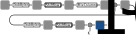
\includegraphics[width=0.8\textwidth, center]{2_goodPractices/figures/aesLastRounds.pdf}
    \caption{Two last rounds of an AES-128}
    \label{fig:aesLastRounds}
\end{figure}
    As we said before, the attack requires single bit faults on AES computation.
    More specifically, the fault has to appear at the beginning of the final AES round.
    Because we are using an AES-128, we will describe everything with this in mind.
    In addition to this, the various notations we will be using are the following:
    \begin{itemize}
        \setlength\itemsep{-0.1em}
        \item $P$ is the AES plaintext and $K$ the AES secret key
        \item $P^i$ stands for the intermediate cipher result after the $i^{th}$ AES round
        \item $P^i_j$ is the $j^{th}$ byte of $P^i$
        \item $K^i$ represents the $i^{th}$ AES round key
        \item As for $P$, $K^i_j$ is the $j^{th}$ byte of $K^i$
        \item $C$ is the correct ciphertext, $C_j$ is the $j^{th}$ byte of C
        \item Eventually, $CF$ stands for the faulty ciphertext, $CF_j$ is the $j^{th}$ byte of CF
    \end{itemize}
    Although the attack requires single bit faults on the final round, the attack is fairly simple and quick to perform with the right data at hand.
    I will not describe how AES operates, as it is well described in \cite{giraudDfa, aesRijndaelProp}.
    The final ciphertext is given thanks to the following equation:
    \begin{equation}
        C = ShiftRows(SubBytes(P^9)) \oplus K^{10}
    \end{equation}
    With $SubBytes(P^i_j)$ being the substitution table (S-box) result calculated on $M^i_j$ byte, and $ShiftRow(j)$ being the $j^{th}$ byte position of the temporary result of the $ShiftRows$ transform.
    \textcolor{orange}{To finish.}

    \subsection{Integrated circuits target characteristics \ddc}
    For the purpose of understanding clearly how we set up the previous attack, it is required to describe thoroughly the integrated circuit targeted.
    The model is an STM32F439VIT6 32-bits ARM Cortex-M4 microcontroller from STMicroelectronics, available in a LQFP100 package.
    The IC is manufactured using a 90 nm bulk technology.
    Its main characteristics are the following:
    \begin{itemize}
        \setlength\itemsep{-0.1em}
        \item A core clock up to 180 MHz
        \item Two 1 MB FLASH memory banks
        \item 256 kB of RAM
        \item Voltage supply allowed from 1.7 V to 3.6 V
        \item A True Random Number Generator (TRNG)
        \item A dedicated hardware cryptographic coprocessor, embedding AES (128, 192 and 256 bits), triple DES, and various HASH algorithms
    \end{itemize}

    \subsection{Preliminary attack experiments \ddc}
    For the purpose of accelerating and simplifying the attack process, especially because creating single bit faults is a troublesome process, I designed experiments, to be conducted on the IC target, allowing me to spot interesting IC areas to perform the attack.
    Because the attack targets the AES coprocessor, all the experiments described here are performed specifically on the AES core area.
    % !TeX root = ../0_Manuscript.tex
%    trim={left lower right upper}
%\begin{figure}[H]
%    \centering
%%    \includegraphics[width=0.5\textwidth,
%%    trim={20cm 0cm 0cm 0cm},
%%    center]{2_goodPractices/figures/aesFastImpGnd.pdf}
%    \includegraphics[width=0.8\textwidth, center,
%    trim={14.9cm 0cm 0cm 0cm}, clip]{2_goodPractices/figures/aesFastImpGnd.pdf}
%    \caption{Fault susceptibility map analysis}
%    \label{fig:giraudFSM}
%\end{figure}

\begin{figure}[H]
    \centering
    \begin{subfigure}{0.49\textwidth}
        \includegraphics[width=\textwidth, center,
        trim={14.9cm 0cm 0cm 0cm}, clip]{2_goodPractices/figures/aesFastGndOnly.pdf}
        \caption{FAM: state-of-the-art}
        \label{fig:gndFSM}
    \end{subfigure}
    \begin{subfigure}{0.49\textwidth}
        \includegraphics[width=\textwidth, center,
        trim={14.9cm 0cm 0cm 0cm}, clip]{2_goodPractices/figures/aesFastImpGnd.pdf}
        \caption{FAM: enhanced}
        \label{fig:giraudFSM}
    \end{subfigure}
    \caption{Fault analysis mapping}
    \label{fig:fam}
\end{figure}

    \textcolor{orange}{To finish.}
